\documentclass{article}
\usepackage[icelandic]{babel}
\usepackage[T1]{fontenc}
\usepackage[utf8]{inputenc}
\usepackage{graphicx}
\usepackage{wrapfig}
\usepackage{subfig}
\usepackage{float}
\usepackage{todonotes}

%Leitað er af myndum í eftirfarandi möppum
\graphicspath{{./technical/}{./sprettir/}}
\linespread{1.5}

\usepackage{graphicx}
\usepackage{wrapfig}
\usepackage{float}

\begin{document}

\tableofcontents
\newpage

\section{Inngangur}
Verkefnið snérist um að búa til kerfi sem greinir
breytingar á gagnasettum í kerfum DataMarket og flagga
frávik frá eðlilegri þróun tiltekinnar tímalínu, sem
gætu bent til þess að um áhugaverðan atburð sé að ræða.

Fyrirhugað er að kerfið okkar verði keyrt innan kerfis
Datamarket og er hugsa þannig að hægt sé að keyra það á
gögnin þeirra hvenær sem er.

Upprunalega var kerfið okkar hugsa þannig að það myndi
athuga hvort ný gögn sem væri verið að bæta við
gangasett Datamarket væru áhugaverð eður ei. Hinsvegar
varð okkur ljóst í þróunnarferlinu að kerfið okkar gæti
gert meira en unnið eingöngu með nýjustu uppfærslurnar
og varð því kerfið okkar yfirgripsmeira ein upprunalega
var hugsað.

\section{Lýsing verkefnis}
Sú þjónusta sem Datamarket veitir er að taka sama töluleg gögn frá opinberum stofnunum og einkaaðilum og gerir þau aðgengileg á einum stað sem og birta þau á auðskiljanlegan máta. Gagnsafn Datamarket er gríðarstórt og fer ört vaxandi. Frá og með 25. janúar 2011 samanstóð það af meira en 13.000 gagnasettum sem innihélt næstum 100 milljón tímalínur. Það gefur augaleið að það er ógerlegt að fara handvirkt í gegnum þetta magn af gögnum til að finna áhugaverða atburði því ætti kerfið okkar að vera kærkomin viðbót við kerfi Datamarket.

Hvert gagnasett hjá DataMarket inniheldur tímaraðir sem
sýna þróun tölulegra stærða yfir tíma. Á hverjum degi
eru tugir, eða jafnvel hundruð slíkra gagnasetta
uppfærð í kerfinu. Hvert gagnasett inniheldur svo að
lágmarki eina, en allt að nokkurþúsund tímaraðir. Sú
þróun sem ein tímaröð sýnir getur verið allt frá vel
þekktum stærðum, s.s. verðbólgu, atvinnuleysi eða
hitastigi í Reykjavík, til mjög sérhæfðra eða jafnvel
undarlegra hluta, eins og innflutningsverðmæti
leðurvara frá Brasilíu!

Mikið er fylgst með þessum algengustu stærðum og
stórvægilegar breytingar í þeim rata iðulega í fréttir
umsvifalaust. En mjög markverð, áhugaverð eða jafnvel
varasöm þróun getur líka birst í stærðum sem fáir
fylgjast með og enginn tekur etv. eftir.

Markmiðið með þessu verkefni er að greina þessi tilvik
sjálfkrafa þannig að hægt sé að beina athygli notenda
DataMarket að þeim. Þannig mætti t.d. hugsa sér að
dregnir yrðu fram á forsíðu DataMarket tenglar á þróun
sem kerfið telur um markverða atburði að ræða.

Verkefnið snýst s.s. um að útbúa aðferðafræði sem er
líkleg til að grípa tilvik af þesu tagi. Tiltölulega
auðvelt er að útbúa mjög gróf algrím sem myndu grípa
mörg tilvik, en líklega einnig leiða af sér töluvert
magn “false positives”. Hugsunin er að byrja á að útbúa
slíka einfalda frumgerð og endurbæta svo aðferðafræðina
eftir því sem reynsla, hugmyndaauðgi og tími gefa
tilefni til.

\newpage

\section{Sprettir}
Verkefnið okkar var þannig lagt upp af DataMarket, að þeir vildu í fyrsta lagi fá heilstætt kerfi sem skilaði niðurstöðum. 
Þær niðurstöður þyrftu þó ekki að verja mjög marktækar og byggja á flóknum reikniaðferðum. Því næst áttum við að þróa reikniaðferðirnar eins 
mikið og mögulegt væri, á þeim tíma sem við höfðum. Þetta verkefni var því mjög opið og ljóst að mikilvægt væri 
af okkar hálfu að halda góðri yfirsýn allan tímann, svo að ekki yrði farið lengra í bætingum en svo að það myndi nást að fullklára þær 
aðferðir sem við ætluðum að hafa í kerfinu, í tæka tíð. Því lögðum við upp með að vinna verkið í tveimur fösum. Áætlunin var þannig að skipuleggja
einungis fyrri fasan í upphafi. Byrja að kynna okkur meðfram þeim fasa hvað við gætum mögulega gert í seinni fasanum, en taka ekki ákvarðanir 
um hvað yrði gert fyrr en í upphafi seinnifasa.

\subsection{Sprettur 0}
Sprettur 0 var settur upp sem undirbúnings sprettur. Ekki voru sögur eins og í hefbundnum spretti, heldur notuðum við þennan tíma til að 
skipuleggja verkáætlun, gerðum áhættugreiningu og unnum að ýmsum öðrum undirbúiningi.
\subsection{Sprettur 1}
Í fyrsta spretti fórum við í að kynna okkur tæknileg atriði sem við ætluðum að nota.
Flest þekktum við, en höfðum ekki unnið með það í Python áður. Þetta voru hlutir eins og prófandrifin þróun, REST-ful þróun og hvernig 
unnið er með JSON skrár. Einnig settum við upp grunn að kerfinu sem gat sótt gögn frá DataMarket. Náðum ekki alveg að kára það sem við lögðum 
upp með og urðum að færa hluta úr sögum yfir í næsta sprett.
\begin{figure}[H]
  \centering
  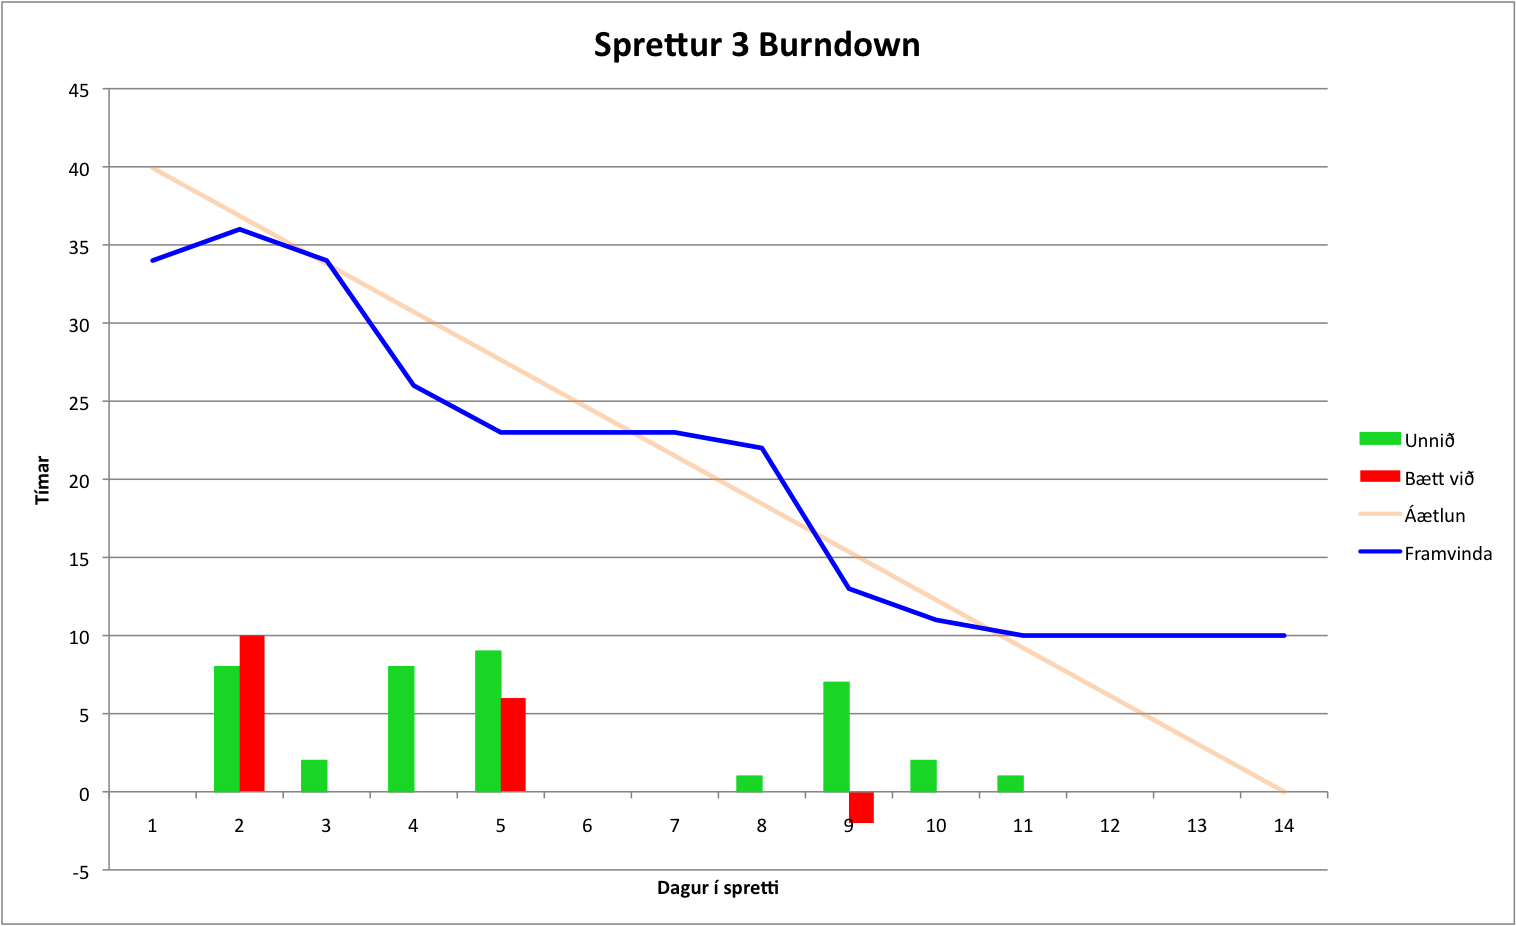
\includegraphics[width=0.72\textwidth]{Sprettur3_Burndown.png}
  \caption{Sprettur 1 Burndown RÖNG MYND}
\end{figure}

\subsection{Sprettur 2}
Í spretti 2 fundum við áhugaverð gögn hjá Datamarket settum upp staðbunda gátt(e.service stub),svo að það myndi ekki hindra okkur í þróun ef 
aðgangur að gagnagrunni Datamarket væri ekki til staðar. Þetta var hluti af okkar áhættugreiningu (VÍSUN í KAFLA). 
Þá bjugum við til fyrstu reikniaðferðirnar, meðaltal miðgildi og staðalfrávik, og létum kerfið sækja gögn og skila niðurstöðum.
Þá áttum við fundi með sérfræðingum á sviði stærðfræði og tölfræði, til að ýta úr vör hugmyndavinnu fyrir seinni fasa.
\begin{figure}[H]
 \centering
 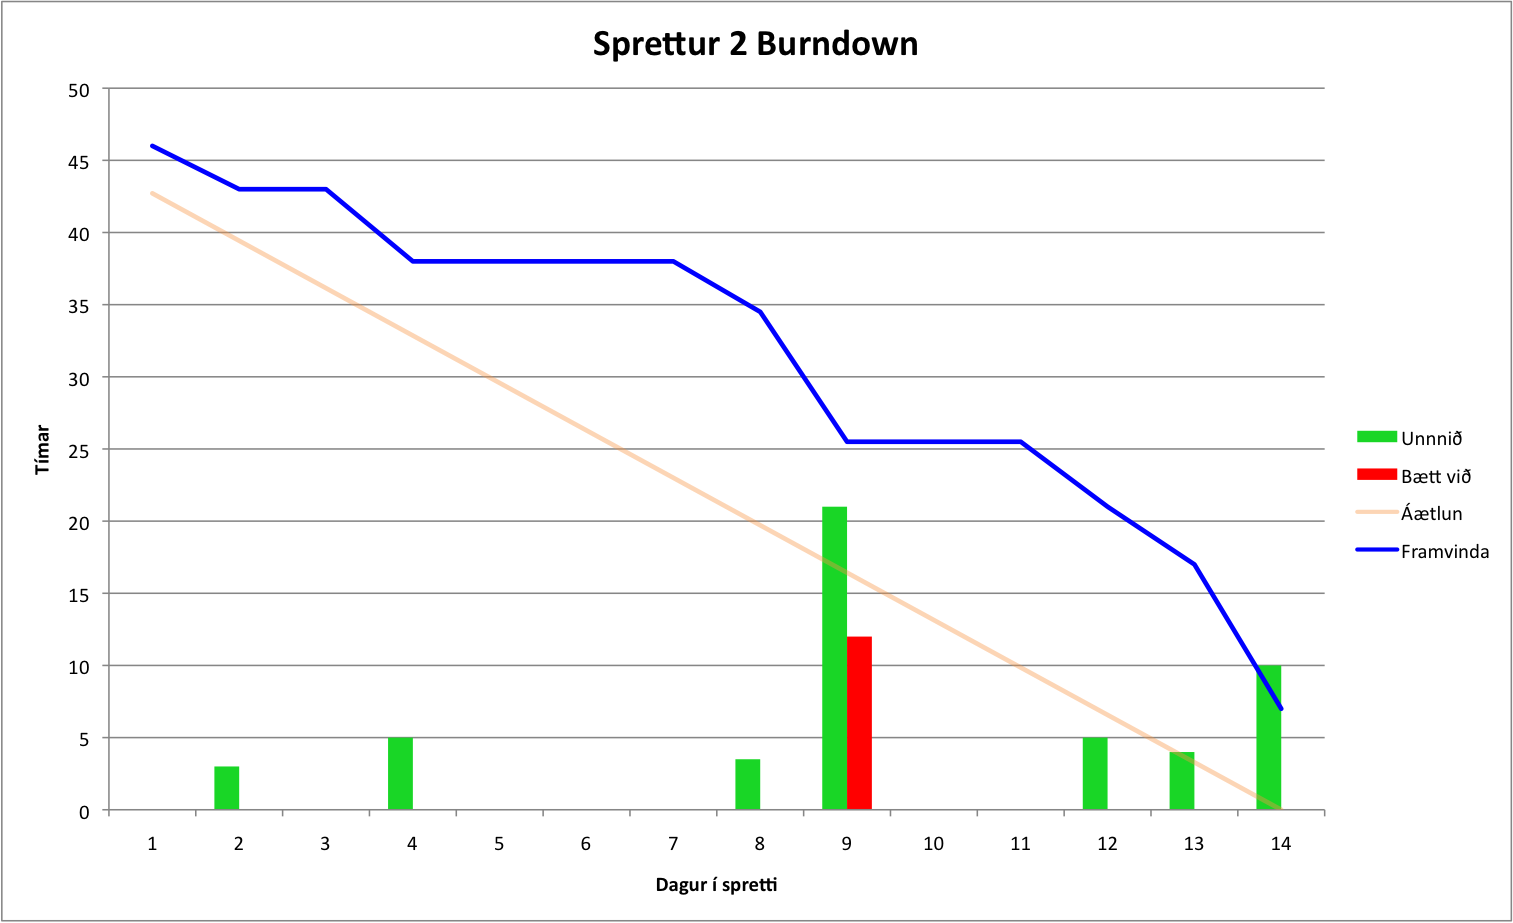
\includegraphics[width=0.72\textwidth]{Sprettur2_Burndown.png}
 \caption{Sprettur 2 Burndown}
\end{figure}
\subsection{Sprettur 3}
Þegar hér var komið við sögu vorum við farnir að finna ákveðinn takt í áætlanagerð og sáum betur hvað við gátum gert ráð fyrir að klára mikið 
í einum sprett. Setum upp aðgerðarsöfn(e. libraries) sem voru til þess fallin að aðstoða okkur við útreikninga. Það tók þó umtalsvert meiri tíma en við gerðum
ráð fyrir. Þá bættum við staðbundnu gáttina og kynntum okkur aðgerðarsöfnin.
\begin{figure}[H]
 \centering
 \includegraphics[width=0.72\textwidth]{Sprettur3Burndown.png}
 \caption{Sprettur 3 Burndown}
\end{figure}
\subsection{Sprettur 4}
Spretturinn fór í að setja upp framenda á kerfið og forma skýrsluna sem það skilar af sér. Þegar við vorum svo farnir að nota aðgerðarsöfnin 
kom á daginn að einföldu aðferðirnar okkar voru mun betri en vonir stóðu til. Einnig komumst við að því að það hafa aðrir beitt þessum aðferðum 
og kallast þær Bollinger bönd ( SJÁ KAFLA UM BOLLINGER BÖND ). 

Við gátum nú sýnt þeim hjá Datamarket niðurstöður úr kerfinu okkar og við það urðu til fleiri hugmyndir um hvernig hægt væri að nýta það ( SJÁ LÝSING VERKEFNIS ).

\begin{figure}[H]
 \centering
 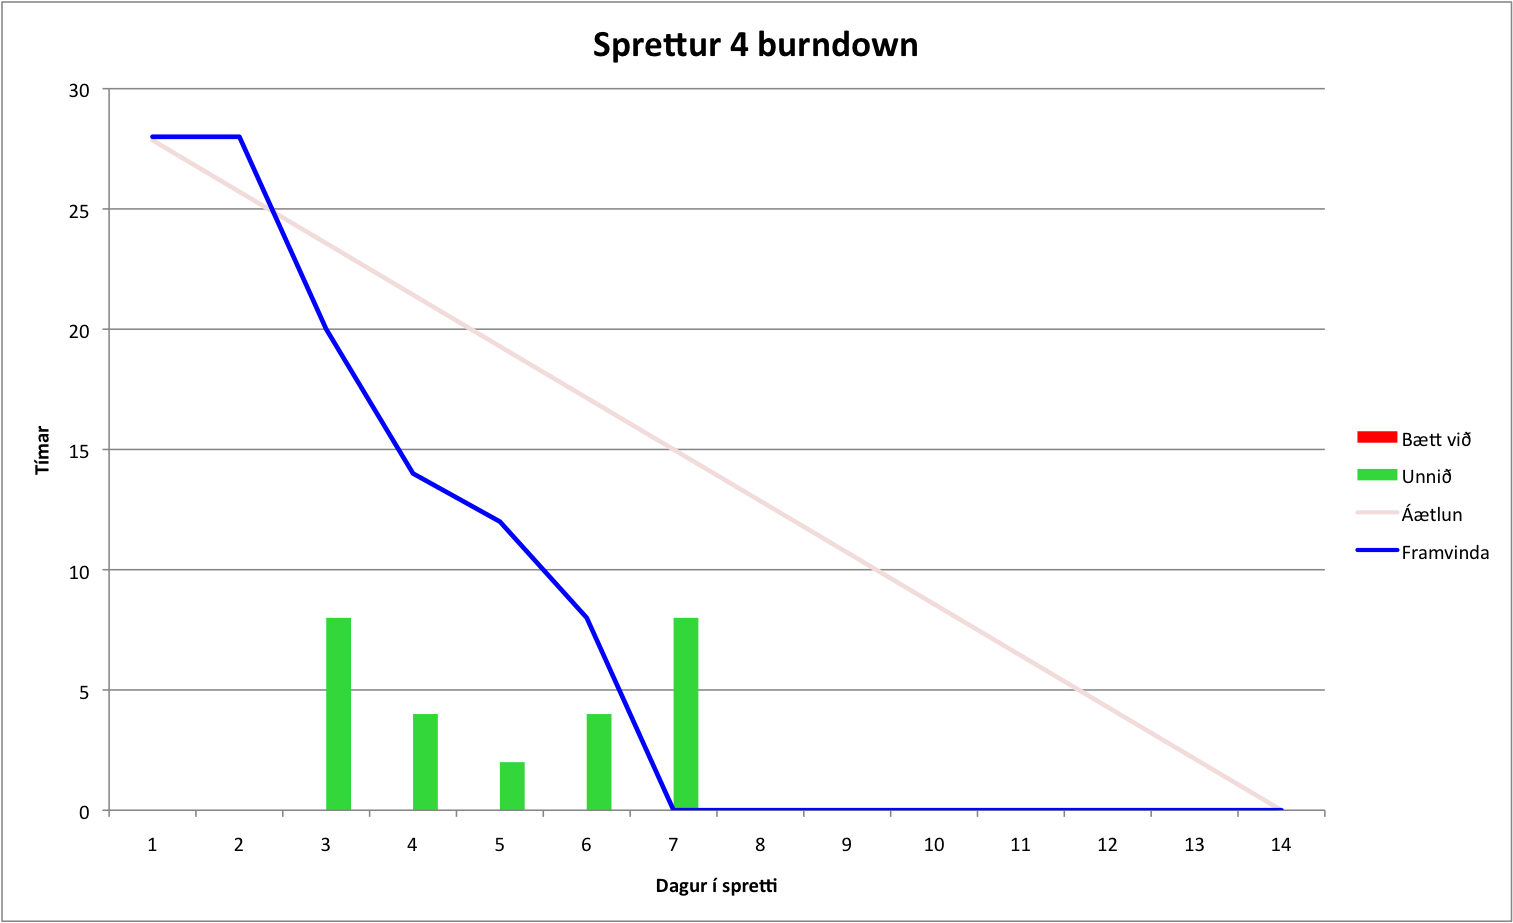
\includegraphics[width=0.72\textwidth]{Sprettur4_Burndown.png}
 \caption{Sprettur 4 Burndown}
\end{figure}

\subsection{Sprettur 5}
Síðasti sprettur í fasa 1. Funduðum með DataMarket og ákváðum endanlegt form á flöggum sem er skilað. Gengum frá lausum endum, og kóði yfirfarinn 
(e. refactor) og útgáfa 1.0 varð til. Hugmyndavinna fyrir fasa 2 komin á fullt.

\begin{figure}[H]
 \centering
 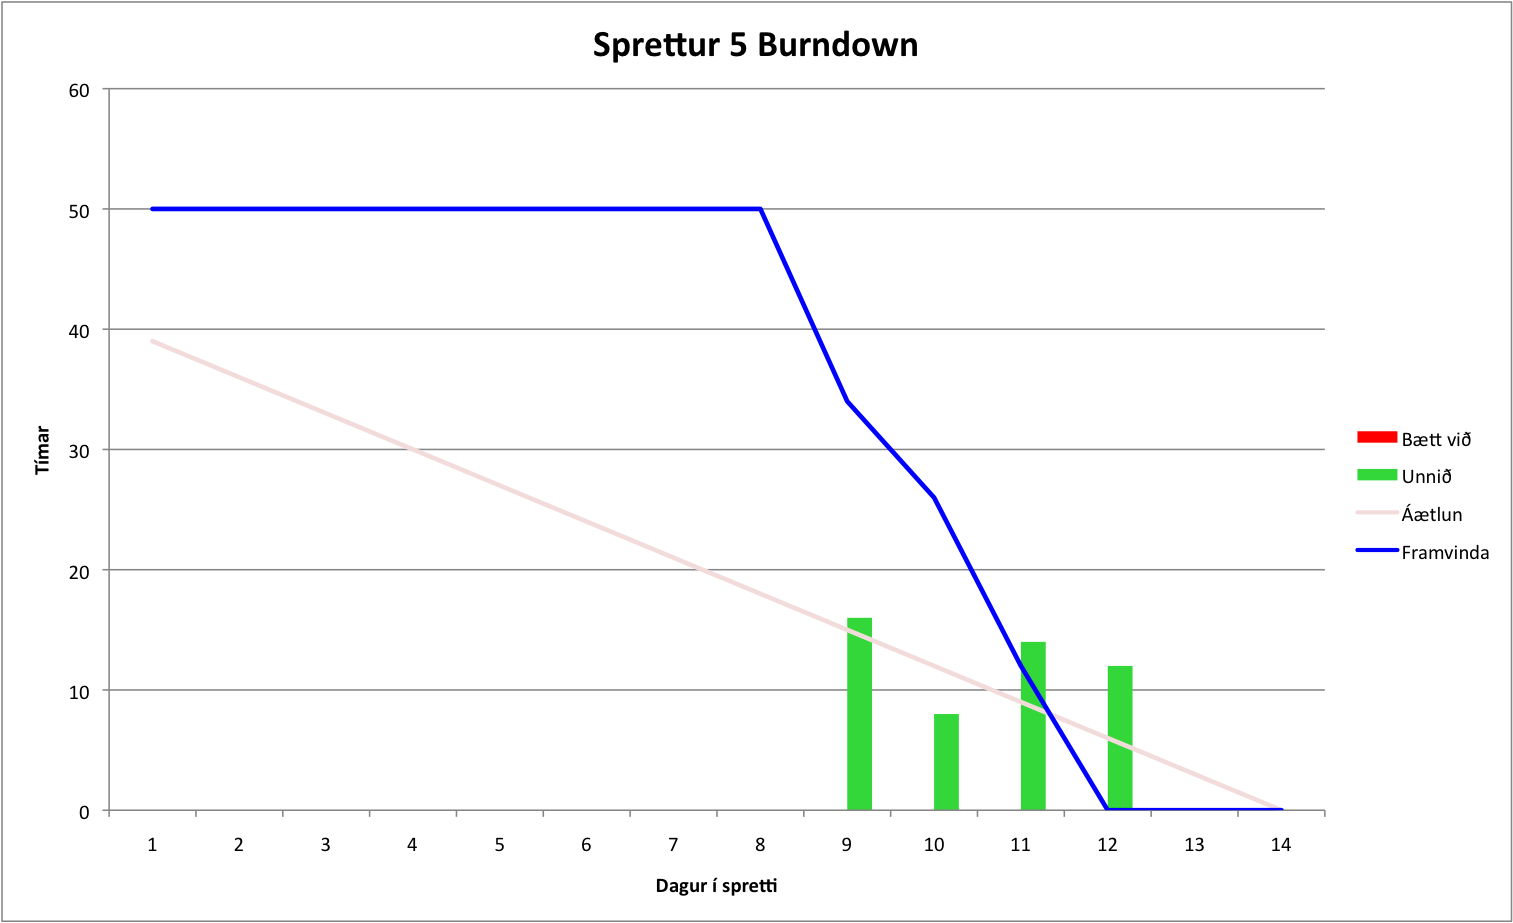
\includegraphics[width=0.72\textwidth]{Sprettur5_Burndown.png}
 \caption{Sprettur 5 Burndown}
\end{figure}

\subsection{Sprettur 6}
Við höfðum sankað að okkur mikið af upplýsingum og höfðum ákveðnar hugmyndir um hvað okkur langaði að gera. Það krafðist þess hinsvegar að við 
þurftum að framkvæma prófanir til að sjá hvað myndi henta okkar kerfi best. Því skipulögðum við sprettinn létt og bættum í hann þegar líða tók á. 
Fljótlega komumst við þó að niðurstöðum um hvaða útfærslur við vildum nota ( SJÁ TÆKNIKAFLA ). Vinna við lokaskýrslu hófst. Í lok sprettsins 
vorum við komnir með verulega bættar reikniaðgeðir frá því sem var.

\begin{figure}[H]
 \centering
 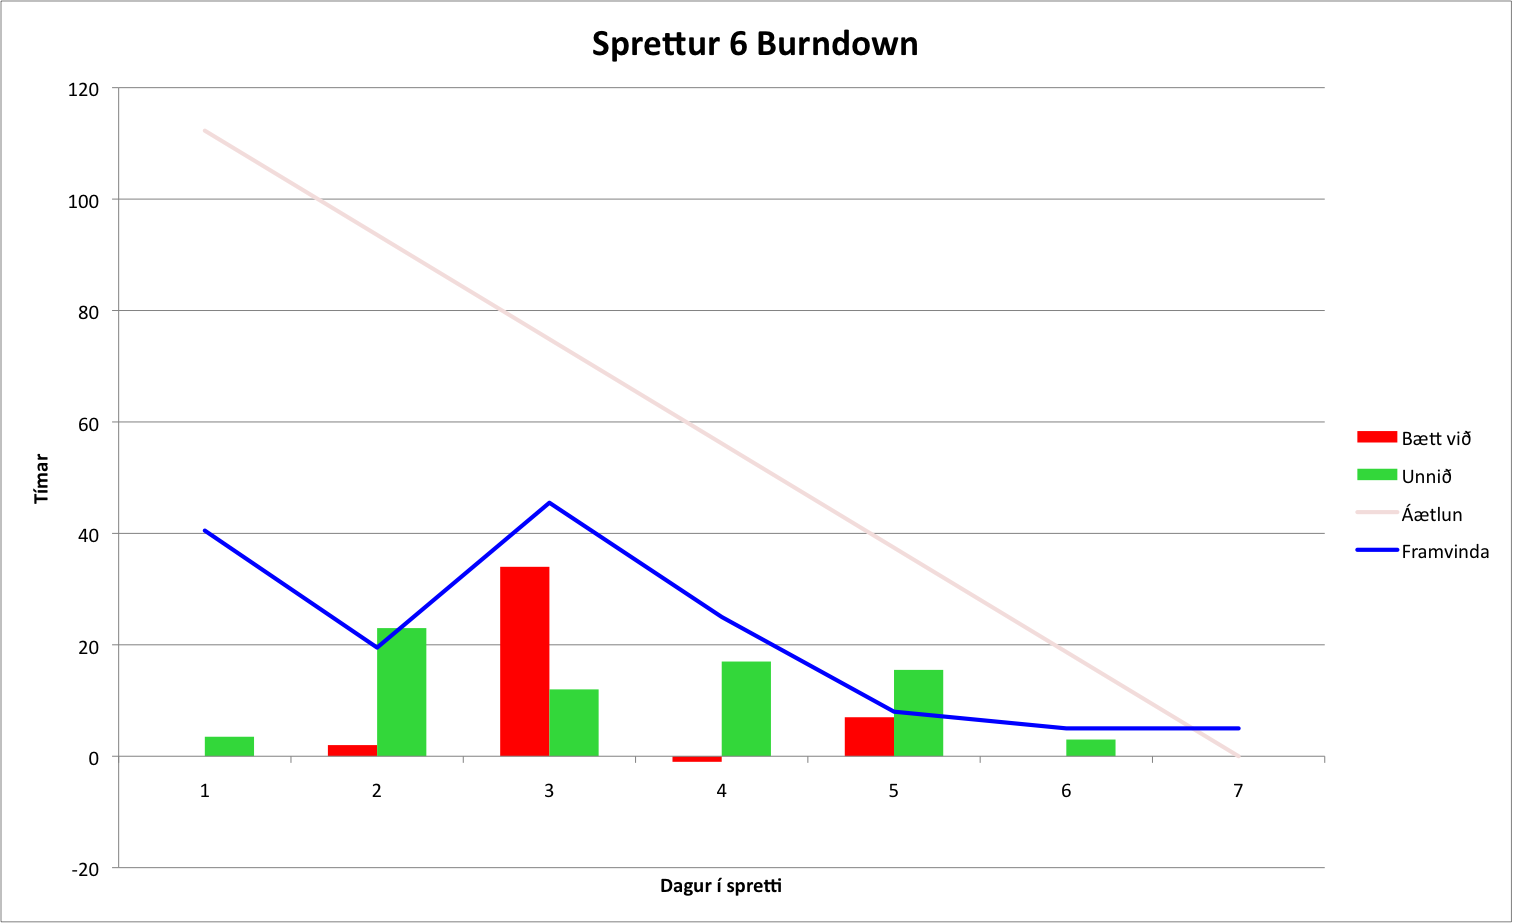
\includegraphics[width=0.72\textwidth]{Sprettur6_Burndown.png}
 \caption{Sprettur 6 Burndown}
\end{figure}

\subsection{Sprettur 7}
Byrjað á lokafrágangi. Allar keyrslustillingar lesnar úr skrá og villumeðhöndlun yfirfarin. Sett upp log kerfi. Álagsprófanir framkvæmdar og 
niðurstöður úr þeim yfirfarnar. Fínstillingar á reikniritum í kjölfar prófanna og villur lagfærðar. 

\begin{figure}[H]
 \centering
 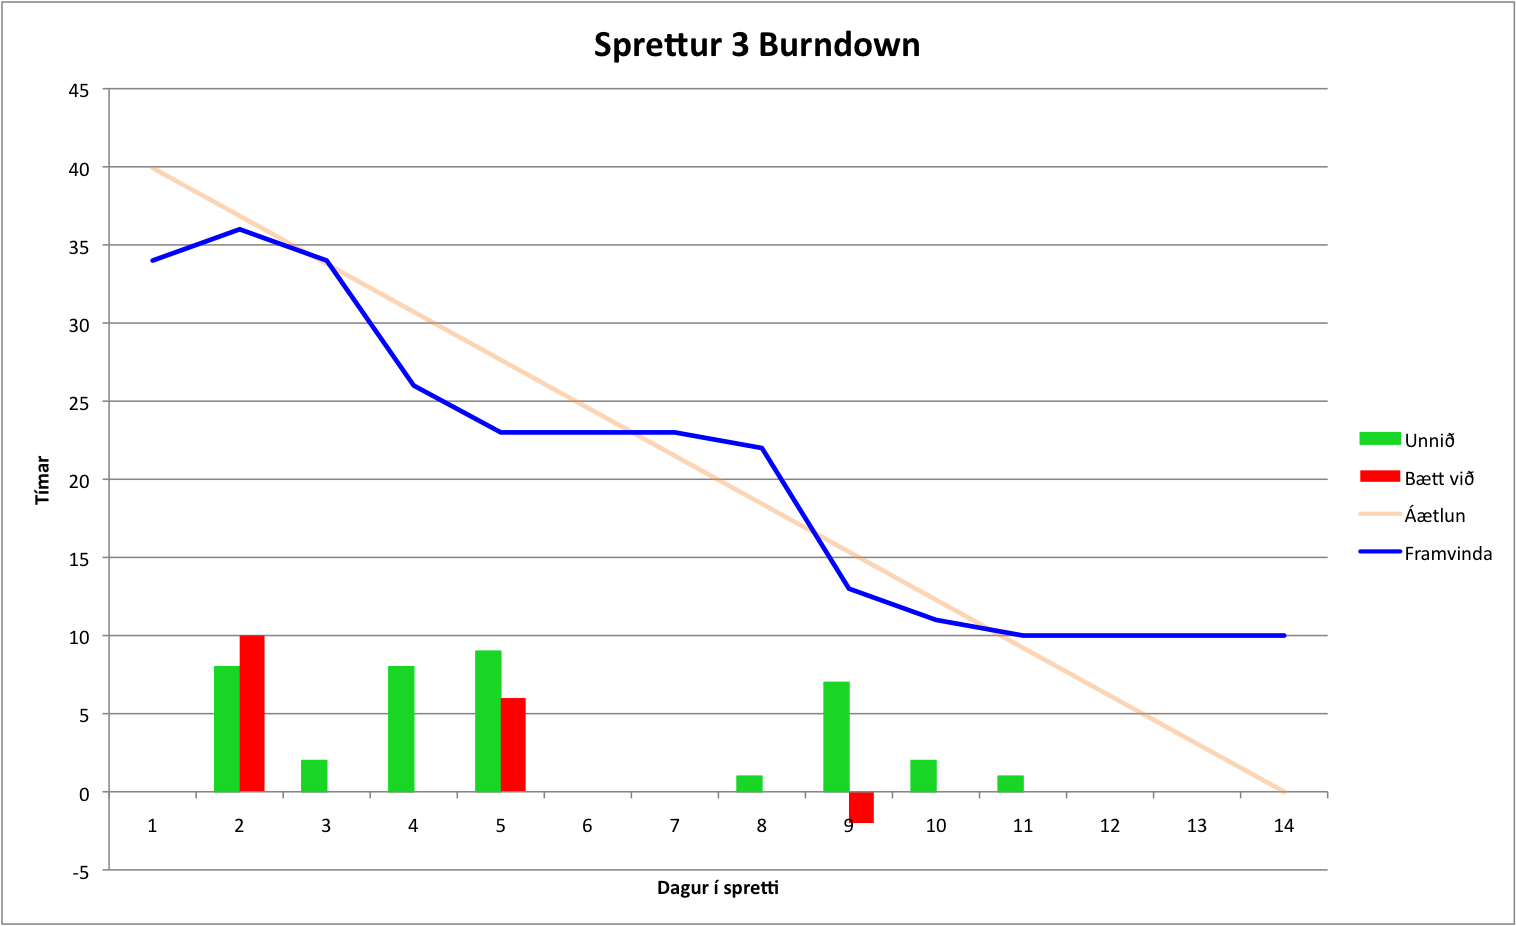
\includegraphics[width=0.72\textwidth]{Sprettur3_Burndown.png}
 \caption{Sprettur 7 Burndown RÖNG MYND}
\end{figure}

\subsection{Sprettur 8}
Skýrslugerð í aðalatriði í lokasprett. Lokafrágangur á kóða. Læddum inn einni bætingu á reikniaðferðum og prófuðum uppá nýtt.
\begin{figure}[H]
 \centering
 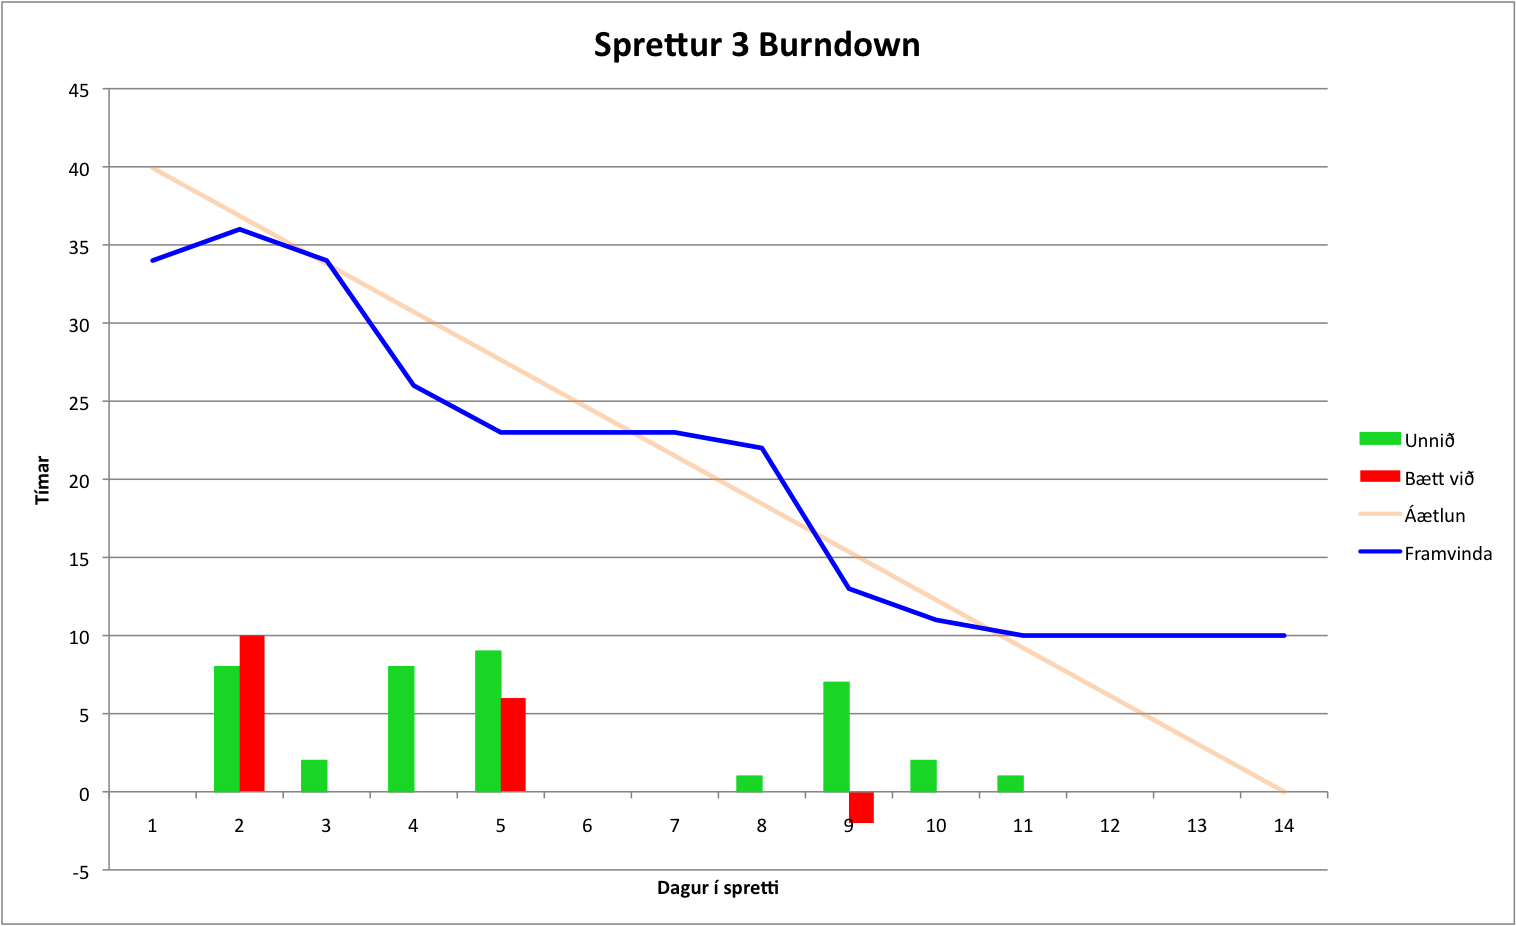
\includegraphics[width=0.72\textwidth]{Sprettur3_Burndown.png}
 \caption{Sprettur 8 Burndown RÖNG MYND}
\end{figure}








\newpage


\section{TækniSkýrsla}


\subsection{Fourier transformations} 

Fourier umbreytingar eru stærðfræðilegar aðgerðir
sem brjóta merki niður í tíðnir þess, slíkt gátum við nýtt okkur með því að láta
umbreyta tímalínu í tíðnir. 
Ef ákveðin tíðni er mjög áberandi í tíðniritinu, þá er að öllum líkindum endurteknging með þeirri tíðni í tímalínunni. 
Sem dæmi um slíkt er tímalínan á mynd~\ref{fig:rafmagnsnotkun} sem sýnir rafmagnsnotkun í ótilgreindu landi.


\begin{figure}[H]
  \centering
    \subfloat[Tímalína]{\label{fig:rafmagnsnotkun}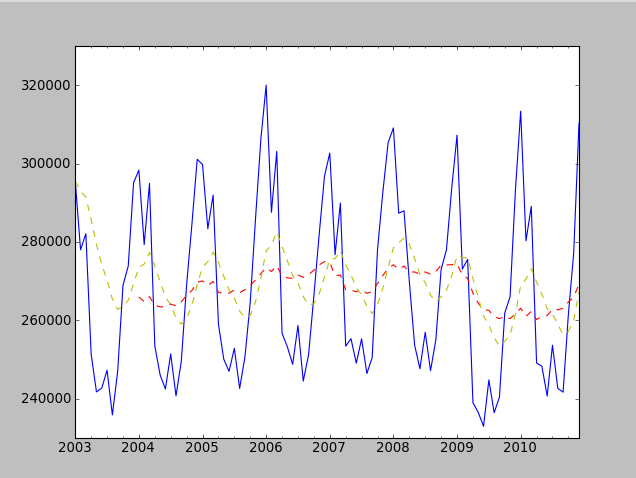
\includegraphics[width=0.42\textwidth]{Rafmagnsnotkun}}                    
    \subfloat[Tíðnirit]{\label{fig:fouriergraph}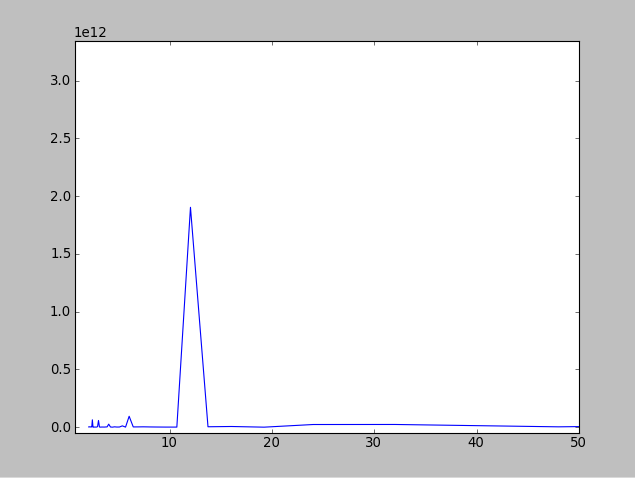
\includegraphics[width=0.42\textwidth]{Fourier}} 
  \caption{Fourier Transformations}
  \label{fig:fourier}
\end{figure}

Það má sjá að tímalínan hefur ákveðnar endurtekningar,
nánar til tekið þá er mikil notkun á veturna en lítil á
sumrin.
Þessa föstu sveiflu í tímalínunni greinir Fourier og
skilar grafi á mynd~\ref{fig:fouriergraph}. 
Úr því er síðan hægt að greina að endurtekning á sér stað með 12 staka millibili.




\subsection{Hlaupandi meðaltal (HM)}
\label{sec:running_average}
Í tölfræði er hlaupandi meðaltal, einnig kallað
fljótandi meðaltal, notað til greiningar á gagnamengi. 
Er það gert með því að mynda röð meðaltala úr
mismunandi hlutmengjum heildarmengisins.
Ef gefin er röð $Z$ talna og ákveðin stærð ramma
(hlutmengis) er $N$, þá er fljótandi meðaltal fundið
með því að fyrst reikna meðaltal 
talna úr sæti $0,1,\dots,N-1$. Þá er ramminn færður
fram um eitt sæti og meðaltal fundið af tölum í sætum
$1,2,\dots,N$. 
Þessi aðgerðarröð er endurtekin yfir alla talnaröðina,
$Z-N$ sinnum.  

\begin{center}
  $HM = \frac{x+(x+1)+\dots+(x+(N-1))}{N}$ 
\end{center}


Línan sem tengir svo saman öll meðaltölin er hið
fljótandi meðaltal þar sem hver punktur á línunni
samsvarar 
meðaltali viðkomandi hlutmengis í heildarmengi ganganna
sem verið er að meta. 
 
\subsection{Vegið hlaupandi meðaltal (VHM)}
\label{sec:weighted_running_average}
Hlaupandi meðaltal getur einnig notað ójöfn gildi fyrir
hvert stak á línunni.
Þá er um vegið meðaltal að ræða og er meðaltalinu gefin
einhver margfeldisáhrif eftir því hvar á línunni það er
staðsett. 
Það vægi breytist línulega. Summu margfeldi allra
gildana í tilteknum ramma er svo deilt með summu allra
mergfeldanna. 
Ef um ramma af stærð 10 er að ræða og gildin eru
margfölduð eftir sætisröð, þá fæst eftirfarandi formúla. 
\begin{center}
  $VHM = \frac{x+2(x+1)+3(x+2)+\dots+(10(N-1))}{1+2+\dots+10}$ 
\end{center}


\subsection{Bollinger bands}
\label{sec:bollinger_bands}

\begin{wrapfigure}{r}{7cm}
%\begin{figure}
 \begin{center}
  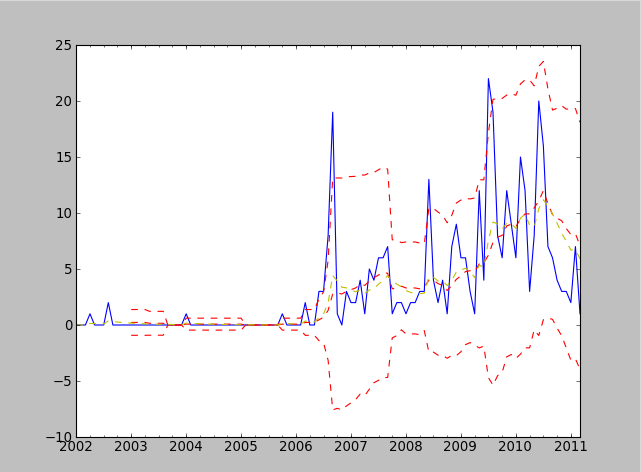
\includegraphics[width=.58\textwidth]{Bollinger.png} 
  \caption{Bollinger bönd merkt með Rauðum strikalínum} 
  \end{center}
%\end{figure}
\end{wrapfigure}

Bollinger bönd eru upprunalega þróuð sem greiningartól
á þróun verðbréfaverða. 
Tilgangur þeirra er að veita viðeigandi skilgreiningu háum og lágum gildum. Einnig hefur þessari 
aðferð verið beitt á ýmis önnur vandamál með misgóðum niðurstöðum. \\
\hfil \\
\hfil \\
\hfil \\
Bollinger bönd samanstanda af:
\begin{itemize}
  \item Miðband, $N-lotu$ einfalt hlaupandi meðaltal.
  \item Efra band, $N-lotu$ staðalfrávik margfaldað með $K$, fyrir ofan miðbandið ($HM + K\sigma$).
  \item Neðra band, $N-lotu$ staðalfrávik margfaldað með $K$, fyrir neðan miðbandið ($HM -K\sigma$).
\end{itemize}


Bollinger bönd nýtast því vel til greininga hvar í
tímalínu óeðlileg hækkun eða lækkun á sér stað.



\subsubsection{Okkar útfærsla á Bollinger}
Útfærslan okkar byggist á því að ítra í gegnum
mismunandi stórar rammastærðir fyrir hverja tímalínu.
Hver rammastærð gefur hverjum punkti einkunn út frá því
hvar punkturinn er staddur með tilliti til Bollinger
bandanna.
Til þess ákváðum við að nota breytta útgáfu af því sem
kallast $\%b$ sem gefur punkti gildi yfir 1 ef
punkturinn er fyrir utan 
efri mörk Bollinger bandsins, tölugildi á bilinu 1-0 ef
punkturinn liggur á milli þeirra og neikvæða tölu ef
hann er undir þeim.

\begin{center}
  $\%b={(last-lowerBB)}{(upperBB-lowerBB)}$
\end{center}

Við notum breytta útgáfu af formúlunni sem hundsar
hvort við erum fyrir ofan eða neðan böndin og gefur
einfaldlega gildi á bilinu
0-1 ef punkturinn liggur á milli bandanna en annars
gildi yfir einum ef punkturinn er fyrir utan. Haldið er
utan um hvort punkturinn 
lá fyrir ofan eða neðan í flagginu sjálfu.

\begin{center}
  $\%b=\frac{abs((item - avg[index])}{(upperlim[index] - avg[index]))}$
\end{center}

Hver rammastærð margfaldar sína útkomu úr formúlunni
við gildið sem punkturinn hefur fyrir.
Þannig gefum við punktum sem líta út fyrir að vera
snörp hækkun í litlum ramma lækkað vægi þegar hann
lendir innan bandanna í stærri ramma
og telst því til eðlilegrar hegðunar þegar horft er
lengra aftur í tímann.
Punktar sem leggja utan Bollinger bandanna í nokkrum
rammastærðum fá einnig aukið vægi þar sem hver rammi
hækkar gildið.

Ef að í tímalínunni er tímabil sem inniheldur svipaðar
eða eins tölur á kafla sem er stærri en rammastærðin er
vandamál að Bollinger 
böndin þrengjast mikið. Það gerði það að verkum að
litlar breytingar eftir þannig tímabil voru gefin
óeðlilega hátt gildi, 
jafnvel töluvert hærra gildi en það sem teldist til
mikið áhugaverðari punkta í sjón. Til að koma í veg
fyrir þetta er notast við
einfalda athugun sem skoðar hvort bandbreiddin fyrir
viðkomandi punkt er óeðlilega þröng miðað við
meðalbandbreidd tímalínunnar.
Ef svo er er punktinum gefið lægra gildi. Þegar þetta
er skrifað er notast við fasta margföldun en hugmyndir
eru uppi um að lækka 
gildið útfrá meðaltali gilda í tímalínunni.

Að lokum hreinsum við flögg sem liggja hlið við hlið,
liggja sömu megin Bollinger bandanna og innihalda
sífellt hækkandi gildi, 
þannig skilum við einungis toppum á hækkunum sem kerfið
sér, en ekki punkta innan hækkunaninnar.













Upprunalega var kerfið okkar hugsa þannig að það myndi athuga hvort ný gögn sem væri verið að bæta við gangasett Datamarket væru áhugaverð eður ei. Hinsvegar varð okkur ljóst í þróunnarferlinu að kerfið okkar gæti gert meira en unnið eingöngu með nýjustu uppfærslurnar og varð því kerfið okkar yfirgripsmeira en upprunalega var hugsað.

Datamarket mun geta nýtt kerfið okkar bæði til að finna áhugaverðust atburðina út úr tilteknum hópi gagnasetta sem og keyrt það á nýjustu uppfærslurnar.

TAKA ÚT Markmiðið með þessu verkefni er að greina þessi tilvik sjálfkrafa þannig að hægt sé að beina athygli notenda DataMarket að þeim. Þannig mætti t.d. hugsa sér að dregnir yrðu fram á forsíðu DataMarket tenglar á þróun sem kerfið telur um markverða atburði að ræða.








\end{document}